

\begin{figure}[t] 
\centering
\newcommand\teaserwidth{0.98}
\subfloat{
    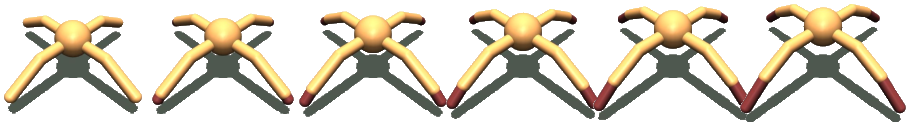
\includegraphics[width=\teaserwidth\linewidth, valign=t]{Figures/teaser/teaser_1.pdf}
}
\\
\subfloat{
    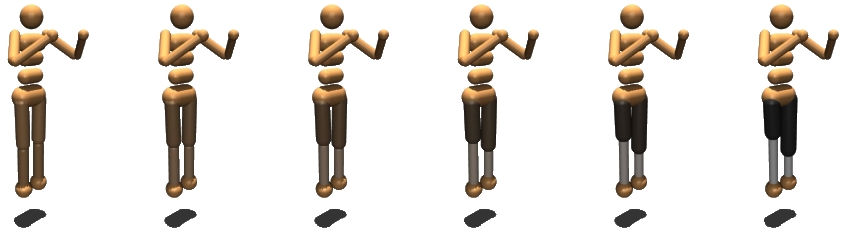
\includegraphics[width=\teaserwidth\linewidth, valign=t]{Figures/teaser/teaser_2.pdf}
}
\\
\subfloat{
    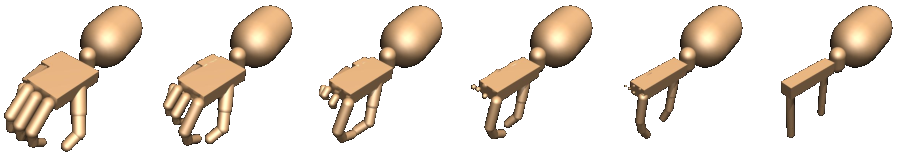
\includegraphics[width=\teaserwidth\linewidth, valign=t]{Figures/teaser/teaser_3.pdf}
}
\caption{ \textbf{Continuous robot evolution model}
allows policy to be transferred from one robot to another robot.
Upper row: an Ant robot continuously grow additional legs from the tip of its feet.
Middle row: a Humanoid robot continuously changes the length and mass of its legs.
Lower row: a dexterous gripper continuously shrink three of its fingers to evolve to a two-finger gripper.
We show the robots at evolution parameters of 0.0, 0.2, 0.4, 0.6, 0.8 and 1.0 respectively from left to right in each row.
}
\label{fig:teaser}
\end{figure}

